\documentclass[11pt]{extarticle}

%% Page Margins %%
\usepackage{geometry}
\geometry{
    top = 0.75in,
    bottom = 0.75in,
    right = 0.75in,
    left = 0.75in,
}

\usepackage{graphicx}
\usepackage{hyperref}

\title{CSC209 Mini-Project - 4-Band Audio Equalizer}

\author{Nathan Bergman (bergma43) & Thomas Sarrazin (sarrazi9)}

\begin{document}
\maketitle

\section{Project Overview}\label{desc}

As music producers and composers, we appreciate having plug-ins to modify our audio however we want. One of the most popular ones is an equalizer (or EQ) which can boost certain frequencies and reduce others. 

The vast majority of software which does this is graphical and can take some time to set up and use. We were looking to find a faster solution. So, our CSC209 project takes the form of a 4-band audio equalizer. 

The user interacts with this program only by executing it with appropriate arguments, in the following format: \texttt{./eq <filename>.wav <effect>}. The user may also input \texttt{./eq mods} for a list of the modifications available in the program.

The program takes in \texttt{<filename>.wav} and returns \texttt{<filename>\_mod.wav} file with modified amplitudes in different frequency ranges (bands) depending on the \texttt{<effect>} selected.

\subsection{A Brief Explanation of Manipulating Audio Data from \texttt{.wav} Files}\label{wav}

One of the more time-consuming parts of this project was understanding how \texttt{.wav} audio data was stored and how we would use it to fulfil our goal with this project. Information on the topic was also surprisingly hard to come by, which is why we include this short summary of the what needed to understand the how of our program. \\

\texttt{.wav} files are separated into two main parts: the metadata (44 bytes long) which contains information about the file, and the audio data itself (the remaining bytes in the file), called \textbf{Pulse Code Modulation Data} (or PCM data for short).

PCM data is stored as a sequence of integers in binary, of which the size depends on a parameter called \textbf{bit depth}. Common values for bit-depth are 16 bits (CD quality), 24, and 32 bits (professional recordings). PCM data effectively acts as samples of audio, or snippets of the wave form of the audio. A \texttt{.wav} file stores a certain number of samples per second, usually at a frequency of $44.1$Khz (if working with audio) or $48$Khz (if working with video). This value is called the \textbf{sample rate}.\\

Wave forms are great, but not quite what we want for this project; we are looking for \textit{frequencies}.

To get frequencies from wave forms, we must convert the time domain into the frequency domain. There are three steps to this process. First, we must normalize the wave forms so that their values are all between $0$ and $1$ (this makes further calculations faster!), Then, we must apply a \textbf{windowing function} to smoothen the samples for use in the final step, when the conversion itself is done using \textbf{Fast Fourier Transforms (FFT)}. These transforms take a certain number of wave forms (usually a power of $2$ for algorithm efficiency) and converts them into frequency bins ranging from $0$Hz to the \textbf{Nyquist frequency}, which is equal to the sample rate divided by two. You can imagine the frequency bins as a ``snapshot" of how loud the audio is at different pitches at a given time.\\

These snapshots are exactly what we are looking for! But once we are done with amplifying them however we want, how do we convert them back to wave forms? The answer to this question is to go through the same steps in reverse order!

We will first want to do an \textbf{Inverse Fast Fourier Transform (IFFT)} on each snapshot to convert all our them back into wave forms. It is then just a matter of putting them back together in a file with metadata, and our audio has been modified!

\subsection{Application Processing Steps}\label{steps}

The amplification process is done through multiple steps, listed below. In our case, the window function we are using is the Hann Window Function, which has the following formula:

$$H(n) = \sin^2\left(\frac{n\pi}{N-1}\right)$$

Where $n$ is the sample's normalized PCM value and $N$ is the number of samples taken in the window (and thus how many are taken in the following FFT and IFFT).

\begin{enumerate}
    \item Fetch metadata and PCM data from the \texttt{.wav} file input (line 76, call to \texttt{parse\_file} from \texttt{parse\_file.c}).
    \item Check which preset was selected by the user (line 84, call to \texttt{select\_bands} from \texttt{audio\_presets.c}).
    \item Normalize PCM data (line 125, call to \texttt{prepare\_data} from \texttt{modify\_data.c}).
    \item Perform FFT on each slice of $2048$ integers (line 180, call to \texttt{fft\_execute} from \texttt{fftw\_helper.c}).
    \item Amplify specific frequency ranges by a given amount (line 181, call to \texttt{amplify} from \texttt{modify\_data.c}).
    \item Perform IFFT on each slice (line 182, call to \texttt{ifft\_execute} from \texttt{fftw\_helper.c}).
    \item Create new \texttt{.wav} file with the same metadata as the original file (lines 335-372).
    \item Write modified data to it and return new file (lines 375-386).
\end{enumerate}

Our project belongs to Category 1: Multi-Process Application Using Pipes, as the structure of audio and the goal of our program fits this wonderfully. Indeed, most audio is in stereo format, meaning that the left and right side (channels) each have their own data, so this already calls for multi-process computations, one for each side. Then, we also decided to perform steps 3-5 in separate children processes to the processes for each audio channel. We are doing this by having a worker pool of 20 workers per channel, for a total of 40 workers. The details regarding relations between these processes is detailed in \hyperref[arch]{Section 3}. Their communications are explained in \hyperref[comm]{Section 4}.

\section{Build and Run Instructions}\label{build}
Our application comes bundled with a \texttt{Makefile}. Running \texttt{make} creates the executable under the name \texttt{eq}. This process also creates \texttt{.o} files, and all of these files (including the program) can be removed using \texttt{make clean}.\\

Note that this project requires an external library, namely FFTW3. The \texttt{Makefile} provided covers this for compiling the program on the teach.cs machine, but may need some tweaking if attempting to compile the program outside of teach.cs. The statement to change is the \texttt{-I/usr/include/mkl/fftw -lmkl\_rt} segment in the LIBS variable, to replace with the location of FFTW3 on your machine. If FFTW3 is in the \texttt{mkl} directory (as it is on the teach.cs machine), you must also include \texttt{-lmkl\_rt}. 

\texttt{eq} takes in the file name of the \texttt{.wav} file to modify and the name of the effect preset to apply, in the format \texttt{./eq <filename>.wav <effect>}, and will return a new file named \texttt{modified.wav} once it is done and does not encounter any errors. If \texttt{modified.wav} already exists before running the program, it will be overwritten. The file must be a \texttt{.wav} file, and must have a 16-bit PCM format. These will be checked in the program when the file is read before performing any data manipulation.

\section{Architecture Diagram}\label{arch}

The details of what data is transferred through which pipes can be found in \hyperref[comm]{Section 4}.

\begin{figure}[h]
    \centering
    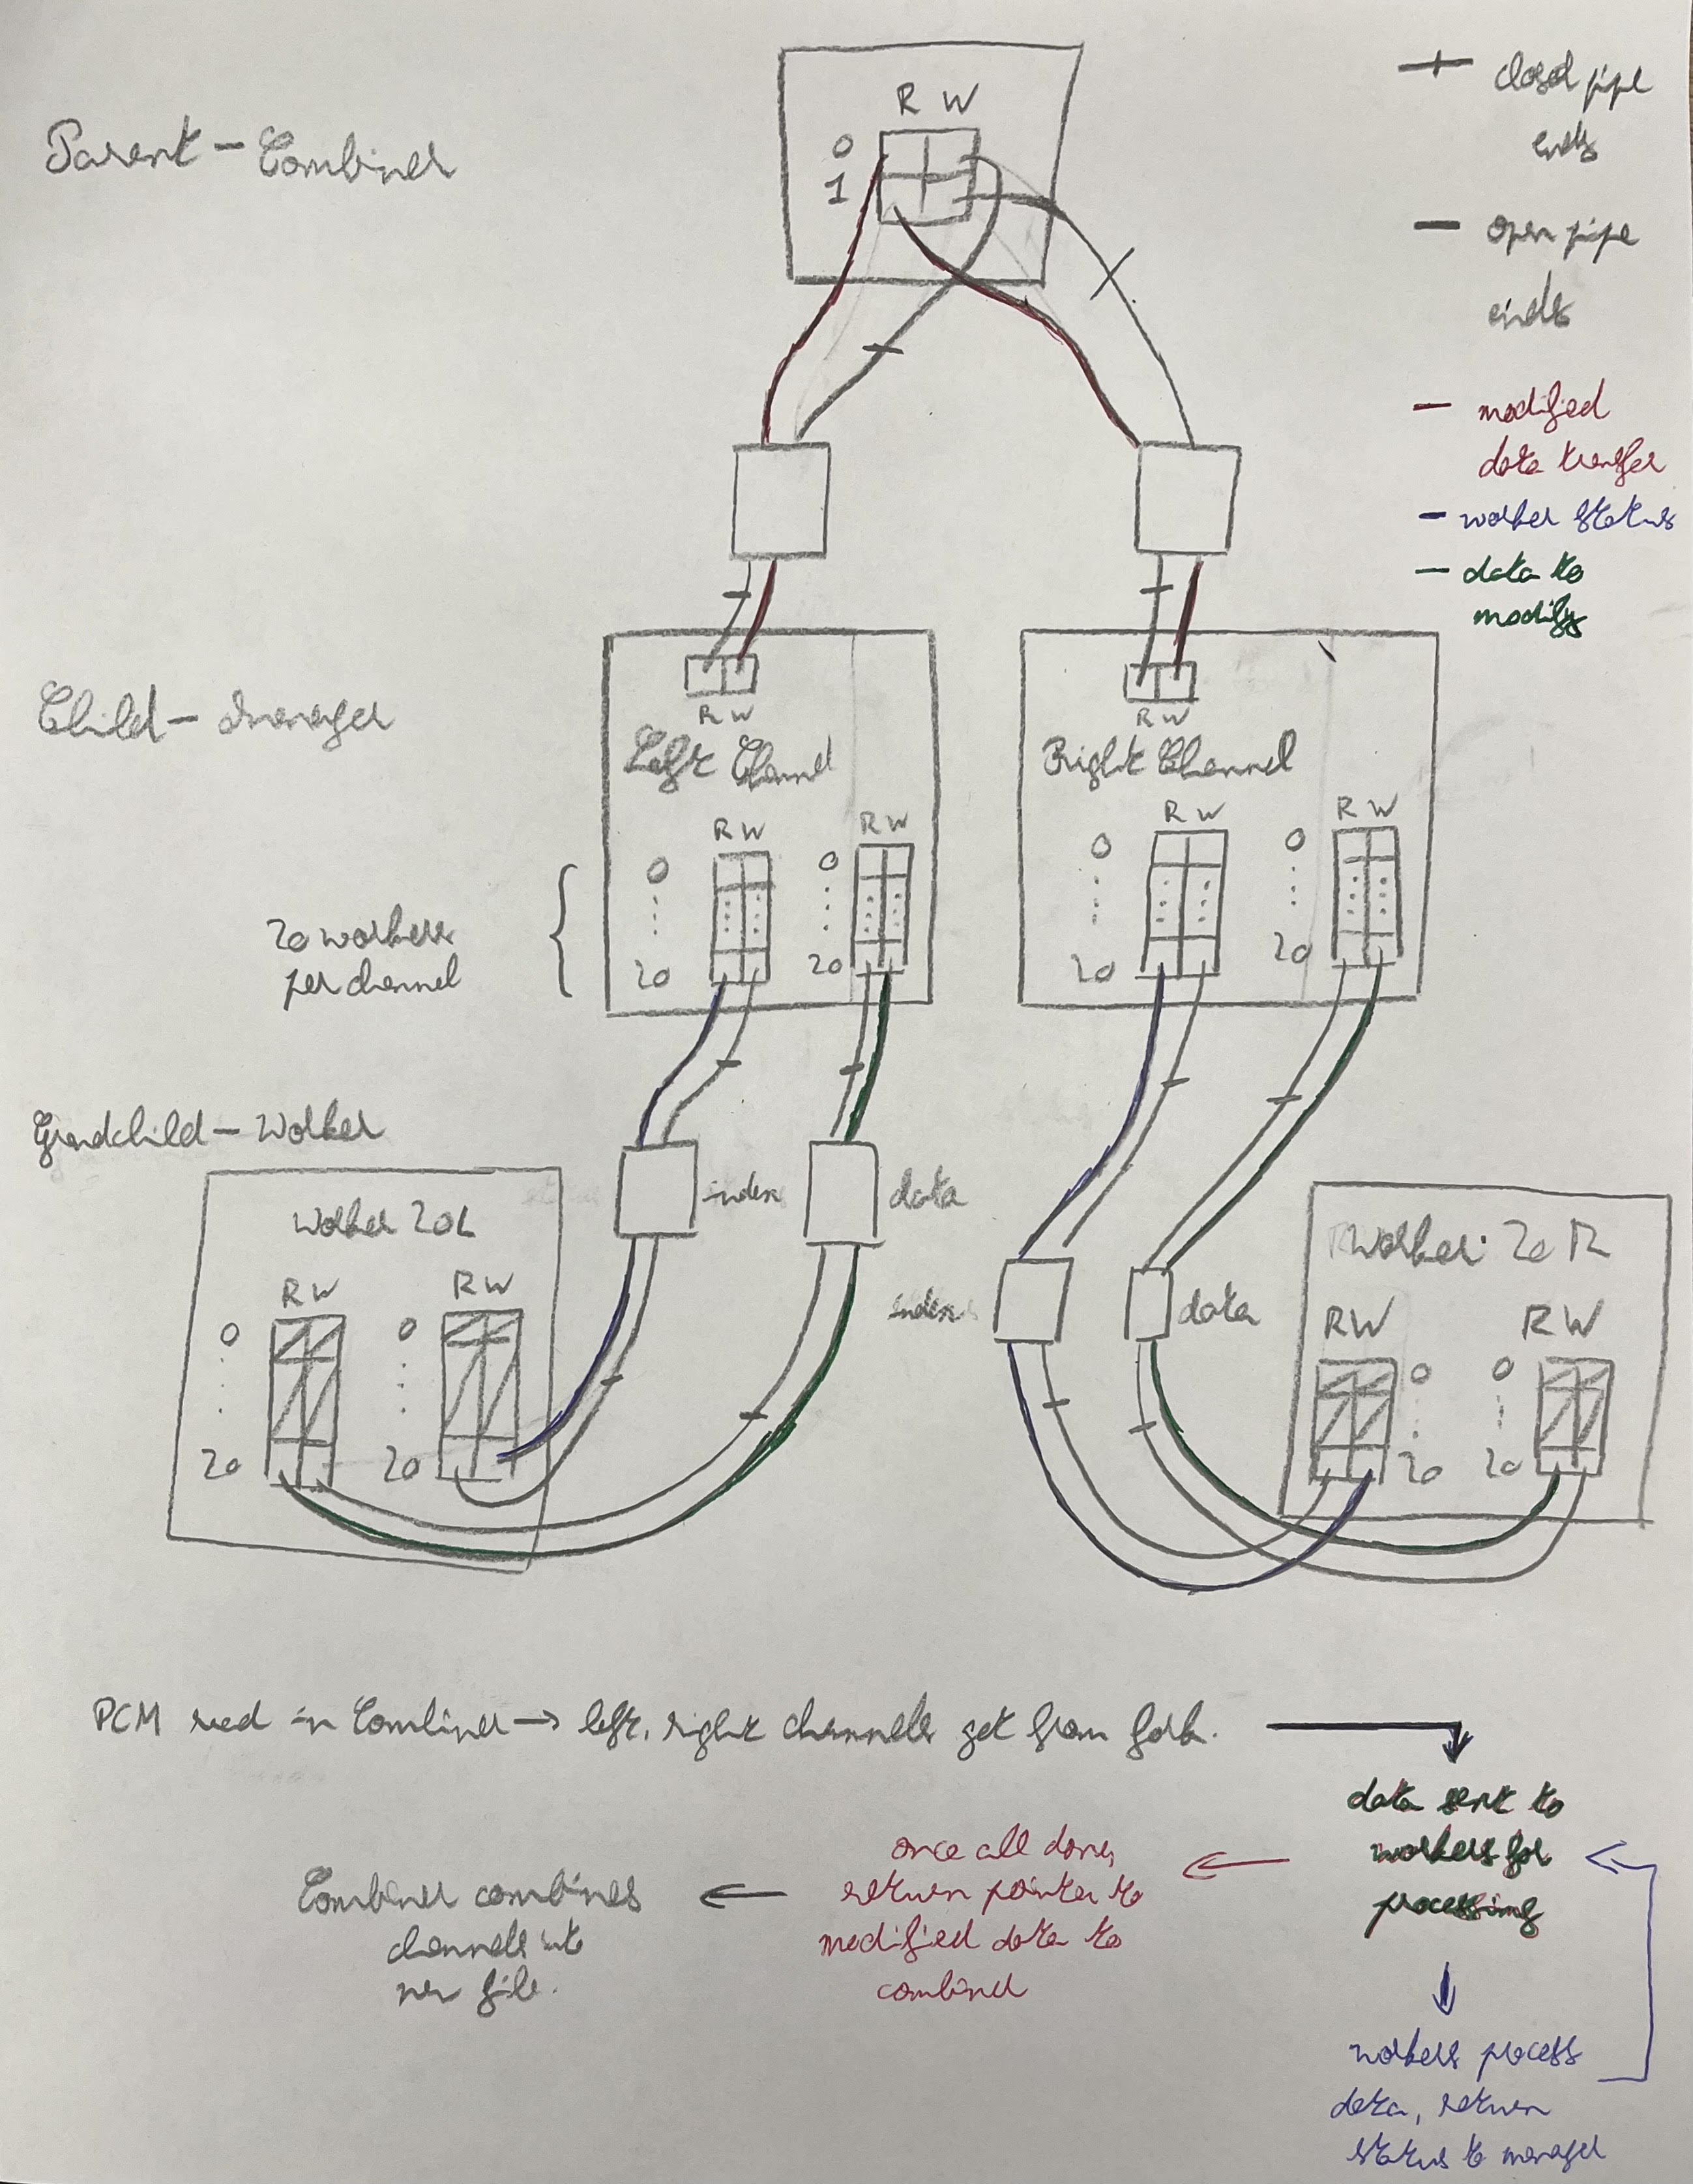
\includegraphics[width=0.7825\linewidth]{architecture.jpg}
    \caption{Architecture Diagram - Combiner-Manager-Worker Model}
    \label{fig:arch}
\end{figure}

\newpage
\section{Communication Protocol}\label{comm}

Our program works on three layers of processes. The top layer we refer to as the Combiner or the parent. The middle layer we refer to as the two Managers or the children. The bottom layer are the Workers, also known as grandchildren. All the communication protocols between these layers are shown in the tables below. \\

\begin{table}[ht!]
\caption{Manager to Worker Communication}
\label{t:MW}
\centering
\begin{tabular}{|l|p{14cm}|}
\hline
Direction & Manager $\to$ Worker \\ \hline
Encoding & Two integers: one for frame number, one for frame size \\ \hline
 Semantics & Instructs workers to process new jobs of size frame size starting at frame number. Upon reading the instructions, the worker does calculations on the frame and gets ready to respond (details below). \\
 & If the work is done, the manager sends -1 as the frame number and the worker shuts down.
 \\ \hline
Error Handling & If an error occurs before the end of the work, the manager sends -1 as the frame number, and the worker shuts down. \\ \hline
\end{tabular}
\end{table}

\begin{table}[ht!]
\caption{Worker to Manager Communication}
\label{t:WM}
\centering
\begin{tabular}{|l|p{14cm}|}
\hline
Direction & Worker $\to$ Manager \\ \hline
Encoding & An integer for frame number and then a series of many bits as the data. The worker keeps writing and the manager keeps reading until either the entire frame is sent or an error message (see details below). \\ \hline
Semantics & Sends completed calculations to the manager for aggregation. The frame number tells the manager where to add the calculations into the results buffer. After reading the results, the manager assigns the next task to the worker, or if the work is done or an error has occurred, a signal to shutdown. \\ \hline
Error Handling & If an error occurs during the calculations, the worker sends -1, signaling the calculations failed on that frame. The Manager then shuts down the program. \\ \hline
\end{tabular}
\end{table}

\begin{table}[ht!]
\caption{Manager to Combiner Communication}
\label{t:MC}
\centering
\begin{tabular}{|l|p{14cm}|}
\hline
Direction & Manager $\to$ Combiner \\ \hline
Encoding & A series of many bits as the data. The manager keeps writing and the manager keeps reading until all of the data is sent (which is determined by number of samples). \\ \hline
Semantics & Sends completed results to the combiner for channel interleaving and writing to a new file. The status number tells the combiner if the calculations were a success. If so, it reads into a buffer, which will then be written to the new audio file. \\ \hline
Error Handling & If an error occurs during the calculations, the manager sends a nonzero status, and the combiner shuts down and does not write anything to the new file. \\ \hline
\end{tabular}
\end{table}

\section{Concurrency Model}\label{conc}

The system for our equalizer is split into multiple depths of forking.

The first depth is from the parent (Combiner) process to the children (Manager, Channel) processes. These are created once the user input has been sanitized (lines 34-73 in \texttt{main.c}) and \texttt{.wav} file is parsed successfully (and related error checks are passed) with a call to \texttt{parse\_file} in line 76 (for which the code is in \texttt{parse\_file.c}), and the modification to perform has been selected (call to \texttt{select\_bands} in \texttt{main.c} lines 83-88. The implementation of the method is in \texttt{audio\_presets.c}). 

The Combiner process waits until both Manager processes have returned to proceed with a \texttt{waitpid} call executed as many times as there are Managers in lines 324-331. If any of Manager processes exit abnormally (which is checked in the aforementioned \texttt{waitpid} call), the program terminates and no file is created.

Manager processes prepare the data for processing with a call to \texttt{prepare\_data} in line 125 before creating pipes and forking Worker processes in lines 142-154. The Managers then continually check for available Workers while there are tasks remaining using the index that they return and a \texttt{poll}. The logic for polling Worker processes until all tasks have been completed is implemented in lines 273-332. Once all tasks have been completed, the Manager writes all of the modified data to its pipe with the Combiner and then collects all its Worker processes by sending an index which causes them to stop waiting for their next task (we decided to make this number -1), in lines 338-352 and 354-366. Once all of this is done, the Manager checks if any Worker processes have exited abnormally one last time. If that is the case, the Manager exits abnormally (which then warns the Combiner and does not create a new file). If the Manager exits normally, the Combiner process then follows its steps to combine the data into a new file.

\section{Error Handling and Robustness}\label{err}

Throughout the steps of our audio processing, there are many checks that we have to make to ensure that the program handles failing appropriately.\\

A crucial step in error checking is first ensuring validity of command-line arguments. We have two arguments to check (to the exception of a \texttt{./eq mods} call which is treated separately in lines 48-59): the file to modify and the effect to apply.

Lines 35-38 ensure that a valid number of command-line arguments are given. This is either 2 (if calling \texttt{./eq mods}) or 3 (if calling the program to modify audio). If any other number of arguments is given, the program will terminate before loading any data and print a short message explaining usage to the user.

For the file name, we have agreed upon a 32-character limit as reasonable for a \texttt{.wav} file (which could be in another directory). If the name of the file is longer, the program will terminate before loading any data and explain that the file name is too long in a print statement. Otherwise, the vast majority of error checking with the file happens in \texttt{parse\_file.c}, when \texttt{parse\_file} is called in \texttt{main.c} in line 76. \texttt{parse\_file} will call \texttt{fopen} to open the audio file for reading and ensure that this call did not fail. It will also check that the file extension of the file to read is \texttt{.wav}, as it will otherwise terminate the program before reading anything from the file. Then, for every piece of information to read, \texttt{fseek} and \texttt{fread} are called in tandem to read the metadata of the audio file, located in a 44-byte header at the start of the file. Every time \texttt{fseek} is called, there will be error-checking in case the file is smaller than the required offset (this could happen if the \texttt{.wav} was corrupted and did not contain enough data for the standard 44-byte header of the format). Every time \texttt{fread} is called, we check for failure and terminate the program if there is a failure. Finally, for reading PCM data, the file will be read in a while loop until \texttt{fread} fails. This can happen either when we have reached the end of the file, or an error has occurred. To differentiate between the two, a final check is made to see if the number of loop iterations to fill the PCM data into the \texttt{WAV\_INFO} struct is the same as the number of samples in one channel. If it is, we know that the entire file has been read, and can proceed with processing. Otherwise, we terminate the program and print a statement to the user informing them of the error.

For the effect, the input is limited to the first two characters as that is the size of all the preset abbreviations. This reduced command-line argument is stored in a temporary string and compared to all possible effect abbreviations in the \texttt{select\_bands} call at line 84 in \texttt{main.c} (the code for the method is located in \texttt{audio\_presets.c}). \texttt{select\_bands} is set to return an integer once it is done: 0 for success, 1 for failure. It is possible that the user did not input a valid effect, in which case the input string will be compared to all possible options but no matches will be found, and \texttt{select\_bands} will return 1. This is error-checked in \texttt{main.c} in lines 84-88, and will terminate the process before any modifications are made to audio file data. \\

%The first checks come through when parsing command-line arguments. The program ensures there are no more than 3 arguments including the program name in the format \texttt{./eq <filename>.wav <effect>}. We have a set limit of 32 characters for the file name, and the modification is checked from a list of two-character modification abbreviations. If any of the arguments are invalid for these reasons, the program will terminate abnormally (return 1).

%Otherwise, the program will attempt to parse the \texttt{.wav} file. This is done with the helper functions in \texttt{parse\_file.c} which is dedicated to that. Checks are done to first verify that the file at the specified path exists when calling \texttt{fopen} and has a \texttt{.wav} extension, and \texttt{fseek} and \texttt{fread} checks are done for every call to these functions. This includes reading the parts of metadata our program requires, and the PCM data itself. The file pointer is then closed within the function to ensure it does not remain open for an extended (unnecessary) amount of time. If at any point the function encounters an issue, the program will immediately exit with code 1 to show failure to the process which called it.

Then, every call to pipe in \texttt{main.c} at all depths in our model (see \hyperref[arch]{Section 3}) is error checked. The same is true for any read calls to and from these pipes, in which we check if the entirety of the data we are supposed to read has been read. To take an example, the Worker processes perform a large number of read calls from their pipe with their related Manager to get the number of samples to process and their location within the file (to keep samples in the same order as the original file). Each read call from this pipe may fail or not read the entirety of the data it is supposed to. The first read is error checked in lines 171-176, as it immediately determines if the Worker can be used or not. If there is an error at this point, the Worker process will not modify any of the data it read and not be used for any data processing as it skips the audio modification loop in lines 181-228 and is effectively retired. The Manager can still function with retired workers, as long as there is at least 1 Worker remaining (hence the use of 20 Workers: it is a reasonably large number to ensure that we can afford having multiple Workers retire and still modify the audio data quickly and as expected).

If there is no issue with the initial \texttt{read} calls however, the Worker will proceed with the \texttt{while} loop in lines 181-228 which is where all the audio processing and modification occurs. During these processes, the Worker calls \texttt{write} to send the index of the data it processed, the number of samples in the data it processed, and the processed data itself to its Manager. All of these \texttt{write} calls are error checked in the event that the pipe they are attempting to write to has closed ends, or if they do not write the entirety of the data. In particular, for the data itself which usually contains 2048 \texttt{double} values, the \texttt{write} call is most likely non-atomic. So, we must check for the amount of data written to the pipe especially in that case, since it is more likely for data to be lost than with the other two values, which are guaranteed to be atomic because of their very small size (both one \texttt{int}). We also error check \texttt{read} calls the Worker makes to receive the next pieces of data to process in lines 220-227, exactly like the calls mentioned in the previous paragraph. This time however, if there is an error with the calls, the Worker process will print the error using \texttt{perror} and exit abnormally. This will warn the Manager process that there was an error with a Worker, and will cause it to exit abnormally as well and warn the Combiner. \\

The last error checks are made once all the data has been processed and transferred to the Combiner. We first ensure that the Manager processes exited normally, which may occur if there was an error in any of the Worker processes, if one of the \texttt{read} or \texttt{write} calls on Manager-Worker and Worker-Manager pipes failed, or if any Manager does not write the entirety of the audio data back to the Combiner process once all computations are done (these error checks are performed throughout lines 286-293, 320-327, and all \texttt{read\_full} calls). To do so, the Combiner process calls \texttt{waitpid(\&status)} as many times as there are Managers in lines 391-398, collecting them sequentially before combining the data. We call \texttt{WIFEXITED(status)} in line 393 to check that the Manager exited by itself and not because of an external signal, and that its \texttt{status} is zero. If \texttt{status} is non-zero for any of the Manager processes, the program terminates before creating the new file and warns the user of failure during the computation of amplified audio data. Otherwise, the program continues normally.

\section{A Short Note about \texttt{valgrind}}\label{valgrind}

While we minimized memory leaks throughout developing our code and refined our allocations and freeing after writing all the code, we still have a significant amount of data identified as ``Still reachable" by \texttt{valgrind}. It seems to us as though we are freeing all memory that we allocated, and saw that it was possible for \texttt{valgrind} to identify this type of leak in \texttt{glibc} methods, which would mean that it is out of our control. Leaks could also be caused by \texttt{MKL} which we use for FFTW but is not within our direct control. So, from what we understand, we are freeing all the memory which we directly allocate ourselves, but there are still minor leaks because of \texttt{glibc} and \texttt{MKL}, which are outside of our control. Furthermore, these memory leaks also fit in the category of ``Still reachable" which means that the memory will be freed automatically by the operating system once the program terminates. For this reason, some argue that ``Still reachable" cases are not true memory leaks and are much more acceptable than other loss categories used by \texttt{valgrind}. 

\section{Team Contributions}\label{team}

Here is a list of what each of us did individually, as well as the work we did together:\\

\underline{Nathan:}

I came up with the idea of making an audio equalizer. I took the lead in normalizing and windowing the data. I spearheaded the FFTW research and set up all of its execution helper methods. I was in charge of establishing the manager to worker and worker to manager communication including assigning the jobs and sending over the data of completed jobs. Then, I wrote up the tables in \hyperref[comm]{Section 4} about these communications. I made the outline for our video, designed the code walkthrough slides and presented them. \\

\underline{Thomas:}


I created the majority of this document, with help from Nathan on proofreading. As far as code is concerned, I implemented \texttt{parse\_file.c} and its associated header for retrieving data from \texttt{.wav} files into a dedicated data structure, and worked on some preliminary functions for data modification in \texttt{modify\_data.c} and its associated header. I also implemented the recombination of modified PCM data into the new file in the Combiner process. I also created test \texttt{.wav} files for testing our code on a variety of sample rates and for the Demonstration. Finally, I created and refined the Makefile.\\

\underline{Teamwork:}

While we worked individually on certain tasks, a lot of the work would not have been possible without working together! We planned times to meet up in person to discuss individual progress and work simultaneously over the past weeks to get this project to where it is at now. We also split tasks for better efficiency, while also reviewing each others' progress throughout. We also came up with ideas for presets and implemented them together, and of course had many team debugging sessions.

\section{Appendix}

\subsection{List of Source File Names and Functions Implemented}

\ 

\underline{\texttt{main.c}}\\

Where the top-level processing happens. Makes calls to functions located in all other files.\\

\underline{\texttt{parse\_file.c}, \texttt{parse\_file.h}}\\

Parses the \texttt{.wav} file provided by the user when calling the program.

Methods:
\begin{itemize}
    \item \texttt{parse\_file} - creates a \texttt{WAV\_METADATA} struct containing the necessary information about the file for processing. Calls \texttt{fill\_pcm} to fill the PCM data for both channels (or only the left channel by default if the source audio file is mono). 
    \item \texttt{fill\_pcm} - fills the \texttt{left\_channel\_pcm} and (if audio source is stereo) \texttt{right\_channel\_pcm} attributes of the \texttt{WAV\_METADATA} struct created in \texttt{parse\_file}.
\end{itemize}

\underline{\texttt{modify\_data.c}, \texttt{modify\_data.h}}\\

Contains all the non-FFT data processing steps.

Methods:
\begin{itemize}
    \item \texttt{normalize} - normalizes a sample so that its value is between 0 and 1.
    \item \texttt{hann} - applies the Hann Window Function on a sample. Called by Worker processes in \texttt{main.c}.
    \item \texttt{prepare\_data} - called by a Manager (Channel) process. Calls \texttt{normalize} on the entirety of the PCM data of that channel.
    \item \texttt{amplify} - called post-FFT in a Worker process. Amplifies frequency bins by a given amount determined by the preset identified in user input when calling the program. 
\end{itemize}\\

\underline{\texttt{fftw\_helper.c}, \texttt{fftw\_helper.h}}\\

Contains all the FFT data processing methods.

Methods:
\begin{itemize}
    \item \texttt{initialize} - creates a plan for the FFT and IFFT transformations as per FFTW specifications.
    \item \texttt{fft\_execute} - performs FFT calculations.
    \item \texttt{ifft\_execute} - performs IFFT calculations.
    \item \texttt{deinitialize} - deletes the plans created in \texttt{initialize} once all FFT and IFFT processing is completed.
\end{itemize}\\

\underline{\texttt{audio\_presets.c}, \texttt{audio\_presets.h}}\\

Performs the selection of the amplification preset used in \texttt{amplify} from \texttt{modify\_data.c}.

Method:
\begin{itemize}
    \item \texttt{select\_bands} - compares preset from user input to fixed list of available presets, and creates a amplification array for use in \texttt{amplify}.
\end{itemize}

\subsection{\texttt{WAV\_METADATA} Struct}

This struct is the main source for the necessary data for the program after reading the audio source file. It is more commonly referred to as its \texttt{typedef}, \texttt{WAV\_INFO}. It is defined in \texttt{parse\_file.h} as follows:

\begin{verbatim}
typedef struct WAVE_METADATA {
    short num_channels;
    int sample_rate;
    short bit_depth;
    unsigned int num_samples; // Size of the PCM for one channel
    double *left_channel_pcm;
    double *right_channel_pcm;
    unsigned int pcm_size; // Total size of the PCM for all channels
    int metadata[11]; // 44 bytes of metadata for access when creating the new file
} WAV_INFO;
\end{verbatim}
\end{document}